    \definecolor{one}{HTML}{E52B50}
    %\definecolor{two}{HTML}{fb8072}
    \definecolor{two}{HTML}{80b1d3}
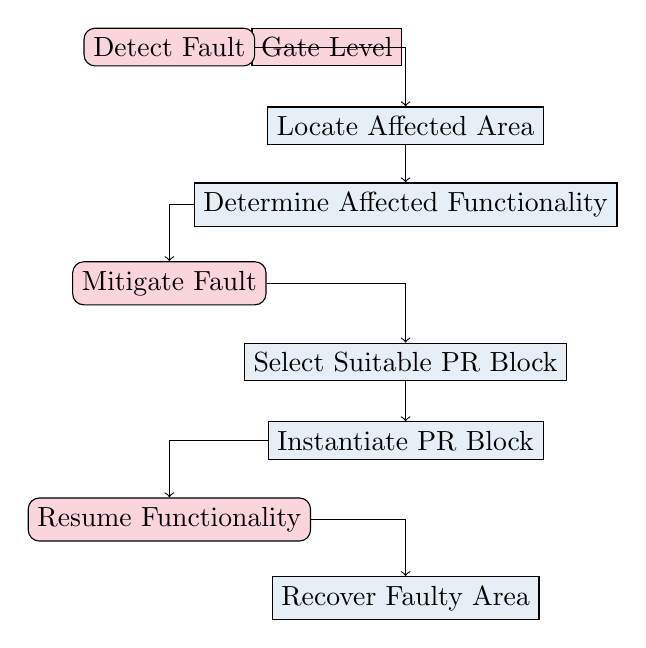
\begin{tikzpicture}[]

\draw[solid]

(0,0) node[fill=one!20, draw] (A) {Gate Level}



(-2,0) node[fill=one!20,draw,rounded corners] (B) {Detect Fault}
(1,-1) node[fill=two!20,draw] (C) {Locate Affected Area}
(1,-2) node[fill=two!20,draw] (D) {Determine Affected Functionality}
(-2,-3) node[fill=one!20,draw,rounded corners] (D1) {Mitigate Fault}
(1,-4) node[fill=two!20,draw] (E) {Select Suitable PR Block}
(1,-5) node[fill=two!20,draw] (F) {Instantiate PR Block}
(-2,-6) node[fill=one!20,draw,rounded corners] (G) {Resume Functionality}
(1,-7) node[fill=two!20,draw] (H) {Recover Faulty Area};
%\draw[dotted] (4, 2) -- (4,-3);
\draw[->, to path={-| (\tikztotarget)}] (B) edge (C);
\draw[->] (C) edge (D);
%\draw[->] (D) edge (E);
\draw[->] (E) edge (F);
%^\draw[->] (F) edge (G);
%^\draw[->] (G) edge (H);
\draw[->, to path={-| (\tikztotarget)}] (D) edge (D1);
\draw[->, to path={-| (\tikztotarget)}] (D1) edge (E);
\draw[->, to path={-| (\tikztotarget)}] (F) edge (G);
\draw[->, to path={-| (\tikztotarget)}] (G) edge (H);
%\draw[->, to path={-| (\tikztotarget)}] (D) edge (E);
%\draw[->] (E) edge (F);
%\draw[->, to path={-| (\tikztotarget)}] (F) edge (G);
%\draw[->] (G) edge (H);
%\draw[->, to path={-| (\tikztotarget)}] (F) edge (G);
%\draw[->, to path={-| (\tikztotarget)}] (G) edge (H);
%\draw[->, to path={-| (\tikztotarget)}] (H) edge (A);
%\draw[->, to path={-| (\tikztotarget)}] (G) edge (B);
%\draw[->, to path={-| (\tikztotarget)}] (H) edge (B);
\end{tikzpicture}
